\section{Design of an Interposition Layer}
\label{arch}

\begin{figure*}[tb]
    \centering
    \subfloat[\label{typical}Typical Experiment Lifecycle]{
        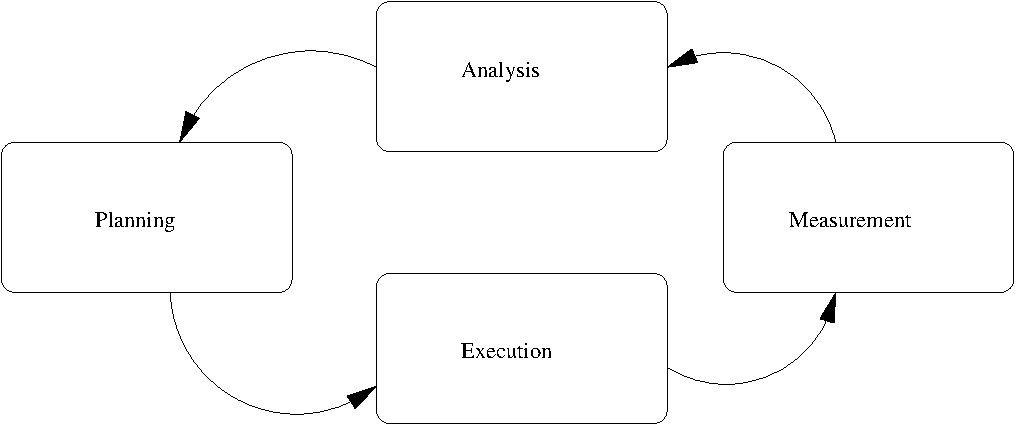
\includegraphics[width=0.4\textwidth]{figs/planning.pdf}
    }
    \hspace{0.5in}
    \subfloat[\label{lem-plan}\name\ Augmented Experiment Lifecycle]{
        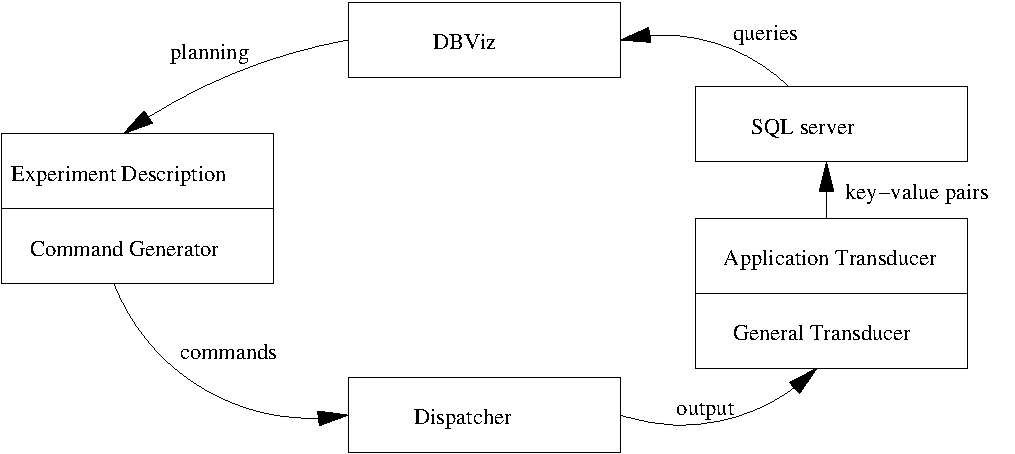
\includegraphics[width=0.4\textwidth]{figs/arch.pdf}
    }
    \mycaption{fig-plan}{Experiment Lifecycle.}{
The figure on the left depicts a typical experiment lifecycle progressing
through planning, execution, measurement, and analysis.  A user devises an
experiment to study the effect of some number of independent variables,
executes and measures each \sub, analyzes the results, and, depending on that
analysis, can then revise the experiment and repeat the cycle.  The figure on
the right shows the workflow within \name.  The user describes their parameter
space to the \cg\ and specifies a path to an optional application transducer to
capture application specific \kv\ pairs.  \name\ adds a path to a general
transducer to capture \kv\ pairs common to all experiments.  The generated
commands and their transducer(s) are then passed to the \dispatcher\ which
either submits the commands to a scheduling system or runs them synchronously
in the foreground.  As the commands run, \kv\ pairs are captured by the
transducer(s) and inserted into a SQL server from which they can then be
queried to visualize and analyze the results.  Depending on this analysis the
user can then modify their parameter space and repeat the cycle.
}
\end{figure*}


We start with the hypothesis that an interposition layer can transparently
rearrange an N-1 checkpoint pattern into an N-N pattern and thereby decrease
checkpoint time by taking advantage of the increased bandwidth achievable via
an N-N pattern. To test this hypothesis, we have developed one such
interposition layer, \plfs, designed specifically for large parallel N-1
checkpoint files. The basic architecture is illustrated in
Figure~\ref{fig-arch}. \plfs\ was prototyped with FUSE~\cite{fuse}, a 
framework for running stackable file systems~\cite{usenix00fist} in 
non-privileged mode.


\plfs\ is a virtual file system situated between the parallel application and
an \upfs\ responsible for the actual data storage. As \plfs\ is a virtual file
system, it leverages many of the services provided by the \upfs\ such as
redundancy, high availability, and a globally distributed data store.  This
frees \plfs\ to focus on just one specialized task: rearranging application
data so the N-1 write pattern is better suited for the \upfs.  In the remainder
of this paper,  we refer to \plfs\ generally to mean this virtual file system
which itself is comprised of a set of \plfs\ servers running across a compute
system bound together by an \upfs; when we refer to a {\em specific} \plfs\ we
mean just one of these servers.

\scribble{Cut last sentence --Milo}

% Although \plfs\ looks and feels like a
%full-fledged parallel file system, in actuality it is merely a collection of
%independent virtual file systems running on each compute node that appear
%parallel only because they exploit the parallelism of the underlying
%file system.

%As multiple processes in a parallel application open an N-1 checkpoint file,

\subsection{Basic operation}
The basic operation of \plfs\ is as follows. For every logical \plfs\ file
created, \plfs\ creates a \Term{container} structure on the \upfs. Internally,
the basic structure of a container is a hierarchical directory tree consisting
of a single top-level directory and multiple sub-directories that appears to
users; \plfs\ builds a logical view of a single file from this container
structure in a manner similar to the core idea of Apple
bundles~\cite{bundles} in Mac OS X.  Multiple processes opening the same
logical file for writing share the container although each open gets a unique
\Term{data file} within the container into which all of its writes are
appended. By giving each writing process in a parallel application access to a
non-shared data file, \plfs\ converts an N-1 write access pattern into a N-N
write access pattern.  When the process writes to the file, the write is
appended to its data file and a record identifying the write is appended to an
index file (described below). 

\scribble{Added words, Mac OS X citation}

\subsubsection{Reading from \plfs}
\label{arch-read}
Rearranging data in this manner should improve write bandwidths, but
it also introduces additional complexity for reads. In order to read 
the logical file, \plfs\ maintains an \Term{index file} for each compute
node which records the logical offset and length of each write. \plfs\ can
then construct a \Term{global index} by aggregating the multiple index files 
into an offset lookup table.

One difficultly in constructing this global index stems from concurrent
processes that may write the same offset at the same time.  These processes
cannot know which will be the ultimate writer, so they need to synchronize to
determine the appropriate order. This synchronization needs to be exposed to
the file system to be effective~\cite{Gibson95thescotch}. If a logical
clock~\cite{lamport1978} was associated with these synchronizations, its value
could be written to index files so that the merge process could correctly
determine write ordering. Since parallel applications synchronize with a
barrier called by all processes, a simple count of synchronization calls could
be sufficient. In practice checkpoints do not experience overlapping writes, so
at this time \plfs\ has not implemented an overlap conflict resolution scheme.

\scribble{changed language on 'serialization of index writes'. We actually only
serialize the index offset updates --Milo} 

One interesting nuance is that \plfs\ has a data file for every process but
only a single index file per compute node shared by all processes on that node.
Sharing an index file is easy; by the time \plfs\ sees writes, they have been
merged by the operating system into a single memory space. The operating
systems sends all writes to a single \plfs\ process which ensures index records
are correctly, chronologically appended.  Having a single index greatly reduces
the number of files in a container since current LANL applications run up to
sixteen processes on a node; on the next LANL supercomputer, this could be up
to sixty-four. We tried reducing the number of data files in the same manner.
Write bandwidth was not affected, but reads were slowed for \Term{uniform
restarts} in which reading processes access the file in the same access pattern
as it was written.  The pattern of a single reader accessing a single data file
sequentially lends itself very well to prefetching.  However, due to timing
differences between the write and read phases, multiple processes in a uniform
restart may not always read from a shared file in sequential order.

Having described the basic operation of \plfs, we now present some of its
implementation in finer detail.  Although there are many interposition
techniques available (~\cite{bypass} includes a survey), we have selected FUSE
for several reasons. Because FUSE allows \plfs\ to be accessible via a standard
file system interface, applications can use it without modification and files on
\plfs\ can be accessed by the entire suite of existing tools such as
\textit{ls}, \textit{diff}, and \textit{cp}. In addition to providing user
transparency, using FUSE dramatically simplified our development effort. A file
system in userspace is significantly easier to develop than a kernel file
system and is more portable as well. However, this convenience is not free as
FUSE does add some overhead as shown in Section~\ref{eval}. 

\subsubsection{Container implementation}

\scribble{I think this part was superfluous so I cut the LD\_PRELOAD stuff}
%Finally, the simplified interface
%of the FUSE API means developers need only implement a small subset of
%function calls as opposed to the much larger set that would be required if
%we had chosen to interpose using an \textit{LD\_PRELOAD} library. As will
%be shown however in Section~\ref{eval}, this convenience is not free as FUSE
%does add some small amount of overhead. 

Because \plfs\ leverages the \upfs\ as much as possible, we give the container
the same logical name as the \plfs\ file. This allows \plfs\ to pass a
\syscall{readdir} system call directly to the \upfs\ and return its result to
the application without any translation.  \plfs\ also handles \syscall{mkdir}
system calls in the same way (\ie\ without any translation). The implication of
leveraging the \upfs\ in this way is that \plfs\ requires some other mechanism
by which to distinguish between regular directories and containers in order to
implement the \syscall{stat} system call correctly. As the \textit{SUID} bit is
rarely used on directories and yet is allowed to be set by the underlying file
system, \plfs\ sets this bit on containers; this does mean, however, that
\plfs\ must disallow setting this bit on a regular directory. 

As we discussed previously, parallel applications do synchronized
checkpointing; the implication for \plfs\ is that multiple processes running on
multiple compute nodes writing an N-1 checkpoint file will cause
\plfs\ on each compute node to attempt to create the same container
concurrently on the \upfs. The difficulty arises because each \plfs\ must first
\syscall{stat} that path to see whether the path is available, whether that
container already exists, or whether there is a regular directory at that
location. Ideally, each \plfs\ could \syscall{stat} the path and, when the
location is empty, atomically create a
directory with the \textit{SUID} bit set. Unfortunately, the \syscall{mkdir}
system call ignores the \textit{SUID} bit; each \plfs\ must therefore first
create a directory and then set the \textit{SUID} bit. Doing this
naively results in a race condition: if one \plfs\ \syscall{stats} the path
after another has made the directory but before it has set the \textit{SUID}
bit, then the \syscall{stat} will indicate that there is a regular directory in
that location. The application issuing the open of the logical file will then
receive an error incorrectly indicating that there is a directory already at
that location. To avoid this race condition, each \plfs\ first makes a
hidden directory with a unique name, set its \textit{SUID} bit, and then
atomically \syscall{renames} it to the original container name.

\subsection{Metadata operations}
\label{arch-meta}

Metadata operations against a file include accessing its permissions (including
SUID), its capacity, the offset of its last byte and the timestamp of its last
update. For a directory on \plfs, these are provided by the underlying
file system. But for a \plfs\ file which is constructed from a container like
the example in Figure~\ref{fig-arch}, these metadata operations have to be
computed from the many underlying files within the container.

Because the SUID bit on the container itself has been overloaded to indicate
that the directory is not a directory at all, but rather a container, it cannot
be also used to indicate if the user has set SUID on the \plfs\ file
represented by the container. Instead we use a file inside the container, the
\Term{access file}, to represent the appropriate SUID and the rest of the
permissions associated with the container. For example, where \syscall{chmod}
and \syscall{chgrp} are directed at the logical file, they are applied to the
access file within the container.

Capacity for the logical file is the sum of the capacities of the files inside
the container.  The last update timestamp is the maximum of the last update
timestamps.  And the offset of the last byte is the maximum logical offset
recorded in any of the index files.

Computing these sums and maximums with every \syscall{stat} call on a \plfs\
file is expensive. Our strategy for speeding this up is to cache recently
computed values in the \Term{metadata subdirectory}. To make this cache as
effective as possible we have each FUSE process cache into this metadata
subdirectory any information it has in its in memory data structures when the
last writer on that node closes the file. On this close, the
FUSE process creates a file named H.L.B.T, where H is the node's hostname, L is
the last offset recorded on that node, B is the sum of the capacity of all
files that this node manages, and T is the maximum timestamp among these files.

When no process has this container open for write, a stat call on the container
is implemented by issuing a \syscall{readdir} on the metadata subdirectory,
then reporting the maximum of the Ls for last byte offset, the maximum of the
Ts for modification timestamp and the sum of the Bs for capacity.

If one or more processes has the container open for writing, then the
corresponding cached metadata values could be stale. \plfs\ clients therefore
create a file in the \Term{openhosts subdirectory} named by its hostname when
one or more processes on that node have that file open for writing, and
then deleting this file once all \syscall{opens} have been closed.
\syscall{stat} must then do a \syscall{readdir} on openhosts as well to
discover if any node has the file open for writing, and thereby determine which
metadata cache entries might be stale.

When there are hostname files in the openhosts subdirectory, the node that is
executing the \syscall{stat} call could read the contents of the index files
associated with those hostnames in order to find the largest logical offset,
and then combine this with the metadata cache files that are not stale.

In the experience of the HPC community, \syscall{stat'ing} an open file is
almost always done by a user trying to monitor the progress of their job. What
they want is an inexpensive probe showing progress, not an expensive
instantaneously correct value~\cite{hec-posix}. Following this logic, \plfs\
does not read and proccess the index files associated with hostnames that have
the container open for write. Instead it assumes that files are not sparse
(\ie\ every byte has been written) and sums the sizes of all data files within
a container to estimate the last offset of the \plfs\ file.  Because writes to
each data are always simply appended, this estimation will monotonically
increase as additional data is written into the file, allowing users to monitor
progress. When the container is closed, the metadata subdirectory contains
fully correct cached values, and full accuracy is provided at all times when
the container has no processes writing it.
